\chapter{Linking Financialization and Urban Productivity} \label{chapter-tramsmission}%{Distribution and Growth} \label{chapter-distribution} % \chapter{Productivity Spillovers}  % \label{chapter-productivity-spillovers}

\epigraph{Alternative micro-foundations cannot be regarded as interchangeable contents for the black box \dots %The micro-foundations of urban agglomeration economies interact with other building blocks of urban models in ways that we cannot recognise unless they are explicitly stated. For instance, the composition of cities typically emerges as a consequence of the scope of different sources of agglomeration economies and their interaction with other aspects of individual behaviour. Third, 
different micro-foundations have different welfare and policy implications. %If we begin building an urban model by postulating an aggregate production function with increasing returns, we can only take this function as given. If instead we derive this aggregate production function from first principles, we may see that its efficiency can be improved upon. The means for achieving such an improvement will depend on the specifics of individual behaviour and technology. Thus, while different assumptions regarding individual behaviour and technology may support similar aggregate outcomes, the normative implications of alternative micro-foundations can differ substantially.
}{Duranton and Puga \cite{durantonMicroFoundationsUrbanAgglomeration2004}}

\epigraph{A large body of literature documents the existence of agglomeration economies in developed economies ... The main conclusion of this literature is the finding of scale economies of 3--8 percent (that is, a 10 percent increase in the size of an activity in a city raises productivity in this activity by 0.3--0.8 percent).}{Gilles Duranton \cite{durantonAreCitiesEngines2009}} % (see Rosenthal and Strange 2004 for a review).



% {\color{red}
% ADD SOME CONTEXT, WHO'S LOOKING AT THIS, WHY ARE THEY INTERESTED IN THIS..  UNLIKE IN  THE OTHER CHAPTERS WEHRE THEREs a unified theroy, in this theory, there are pockets of work  in different fields which to gether make a picture.. 
% CONTEXT AND REFERENCES 

% NEED TO EXPLAIN THE  RELATIONSHIP BETWEEN FINANCIALIZATION AND GROWTH

% AT THE LEAST NEED TO SAY THAT WOULD BE A REASONABLE.

% They money taken out as profit is not reinvested in productivity, human capacity, infrastructure, or consumption. not reinvested.

% Here are the things we know, and here's the reasons we might think this based on the information we have.

% we gather this from xys, putting this together, seeing the trends, it's worth determining

% --- not established in the economic literature, but reasonable too model it.
% }
% %%%%%

%is well approximated by 
Substantial empirical research has shown that the general relationship between population and output at the urban level follows Equation~\ref{eq-agglom-eqn2}: \cite{loboUrbanScalingProduction2013}.\footnote{We use $\beta$ here because it is the most common form in the literature on urban agglomeration, although when we discuss firm production functions we use $\gamma$, $\alpha$ and $\beta$ for the coefficients on capital and labour respectively, as is most common in the economics literature.}

\begin{equation}\label{eq-agglom-eqn2}
    Y=AN^\beta,\qquad \beta>1. 
\end{equation}

 The equation expresses one of the most robust ``stylized facts'' in economics: wealth scales superlinearly with density.  In Chapter~\ref{chapter-growth} we drew on neoclassical growth theory to show that this relationship can be derived from a standard neoclassical firm production function of the form
\begin{equation}\label{eq-producion-fn-eqn2}
    y=AN^\gamma k^\alpha n^\beta,\qquad \alpha+\beta<1. 
\end{equation}
We use Equation~\ref{eq-producion-fn-eqn2} to model the production sector in our model. The model incorporates an agglomeration effect through both $A$ and $\gamma$. We will use the model we explore how financialization enables capital to capture the surplus value produced in cities by agglomeration effects. This capture affects wealth distribution because it shifts surplus value generated by the urban system itself from residents to owners of capital. The shift in wealth is of interest in itself, and it is a feature of the modern urban economy. It may also help explain a significant feature of the empirical results.

Estimates \cite{mccoskeyPanelDataInvestigation, haryantotriRelationshipUrbanizationEducation2021, pugaMagnitudeCausesAgglomeration2010, loboUrbanScalingProduction2013} of  $\gamma$ and $A$ in Equation~\ref{eq-agglom-eqn2} have revealed considerable  variation between regions that has not yet been adequately explained.\footnote{McCoskey and Kao \cite{mccoskeyPanelDataInvestigation} show that the impact of urbanization on growth varies greatly among countries. The World Bank (2016), for example, reported that every 1\% growth in urban population correlates with an increase in GDP per capita by 13\%, 10\%, and 7\% in India, China, and Thailand, respectively. Indonesia realizes only 4\% GDP growth for every 1\% increase \cite{haryantotriRelationshipUrbanizationEducation2021}.  The literature has not yet settled on an explanation of the variation.  \cite{loboUrbanScalingProduction2013, pugaMagnitudeCausesAgglomeration2010} } 
%\subsection{Small cities may provide clues about impact channels }\label{sec-fig-residuals}
Interestingly the residuals or unexplained components for smaller cities are much larger than they are for large cities, as Figure~\ref{fig-residuals-lobo} from Lobo et all \cite{loboUrbanScalingProduction2013} illustrates.\footnote{The observation suggests that clues about the mechanisms may be found by examining smaller and mid-sized cities and that potential policy impacts may be greater for these cities.} 
\begin{figure}[h!tb]
\centering
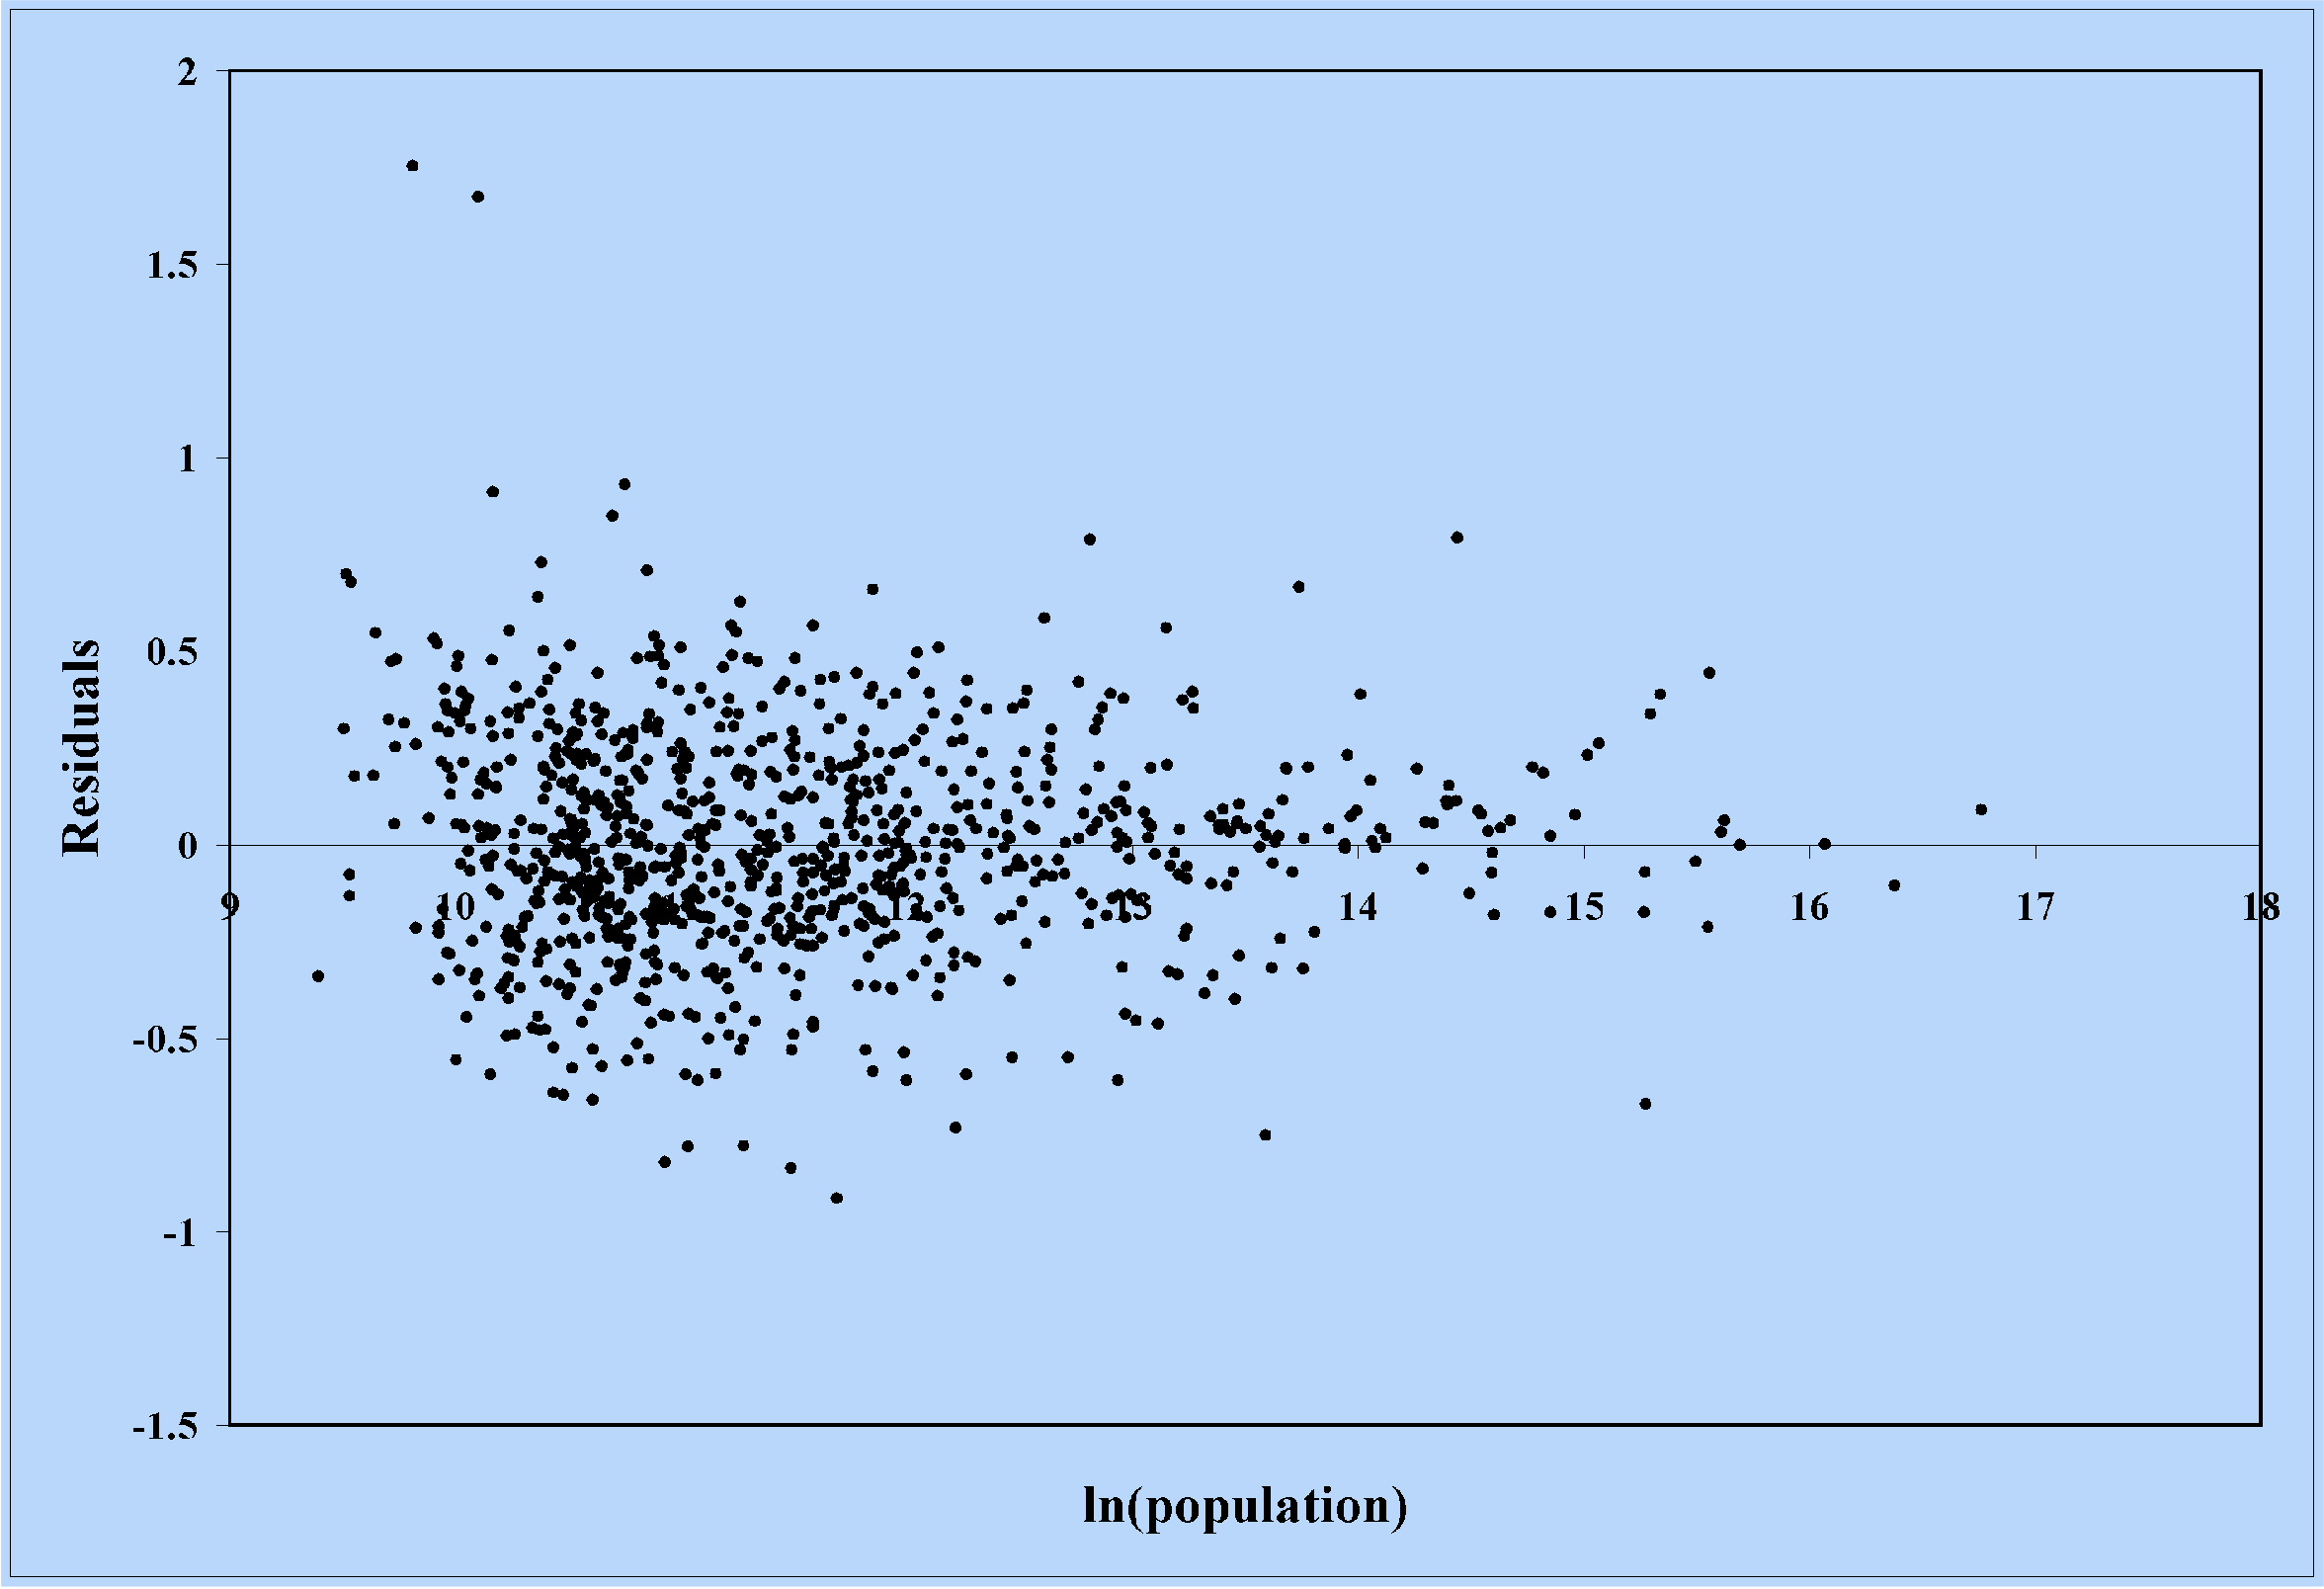
\includegraphics[scale=0.30]{fig/residuals-lobo.png}
\caption{Residuals from regressing ln(total wages) on ln(population) using data for all 943 urban areas of the United States showing larger unexplained components for smaller cities. \cite{loboUrbanScalingProduction2013}.}\label{fig-residuals-lobo}
\end{figure} 
These considerations lead us to consider a new hypothesis: if financialization is redistributing the surplus generated by the growth of the urban system, could it also affect  productivity of the city itself, explaining the variation identified in the scaling literature? 



 %However, there is variation between regions that has not yet been adequately explained.
% {\newpage\thispagestyle{empty}
% \vspace{-1.5cm}
\begin{figure}[h!tb]\label{fig-impact-channels}
%\vspace{-1cm}
\begin{adjustwidth}{-0.24\textwidth}{-0.24\textwidth}
\centering
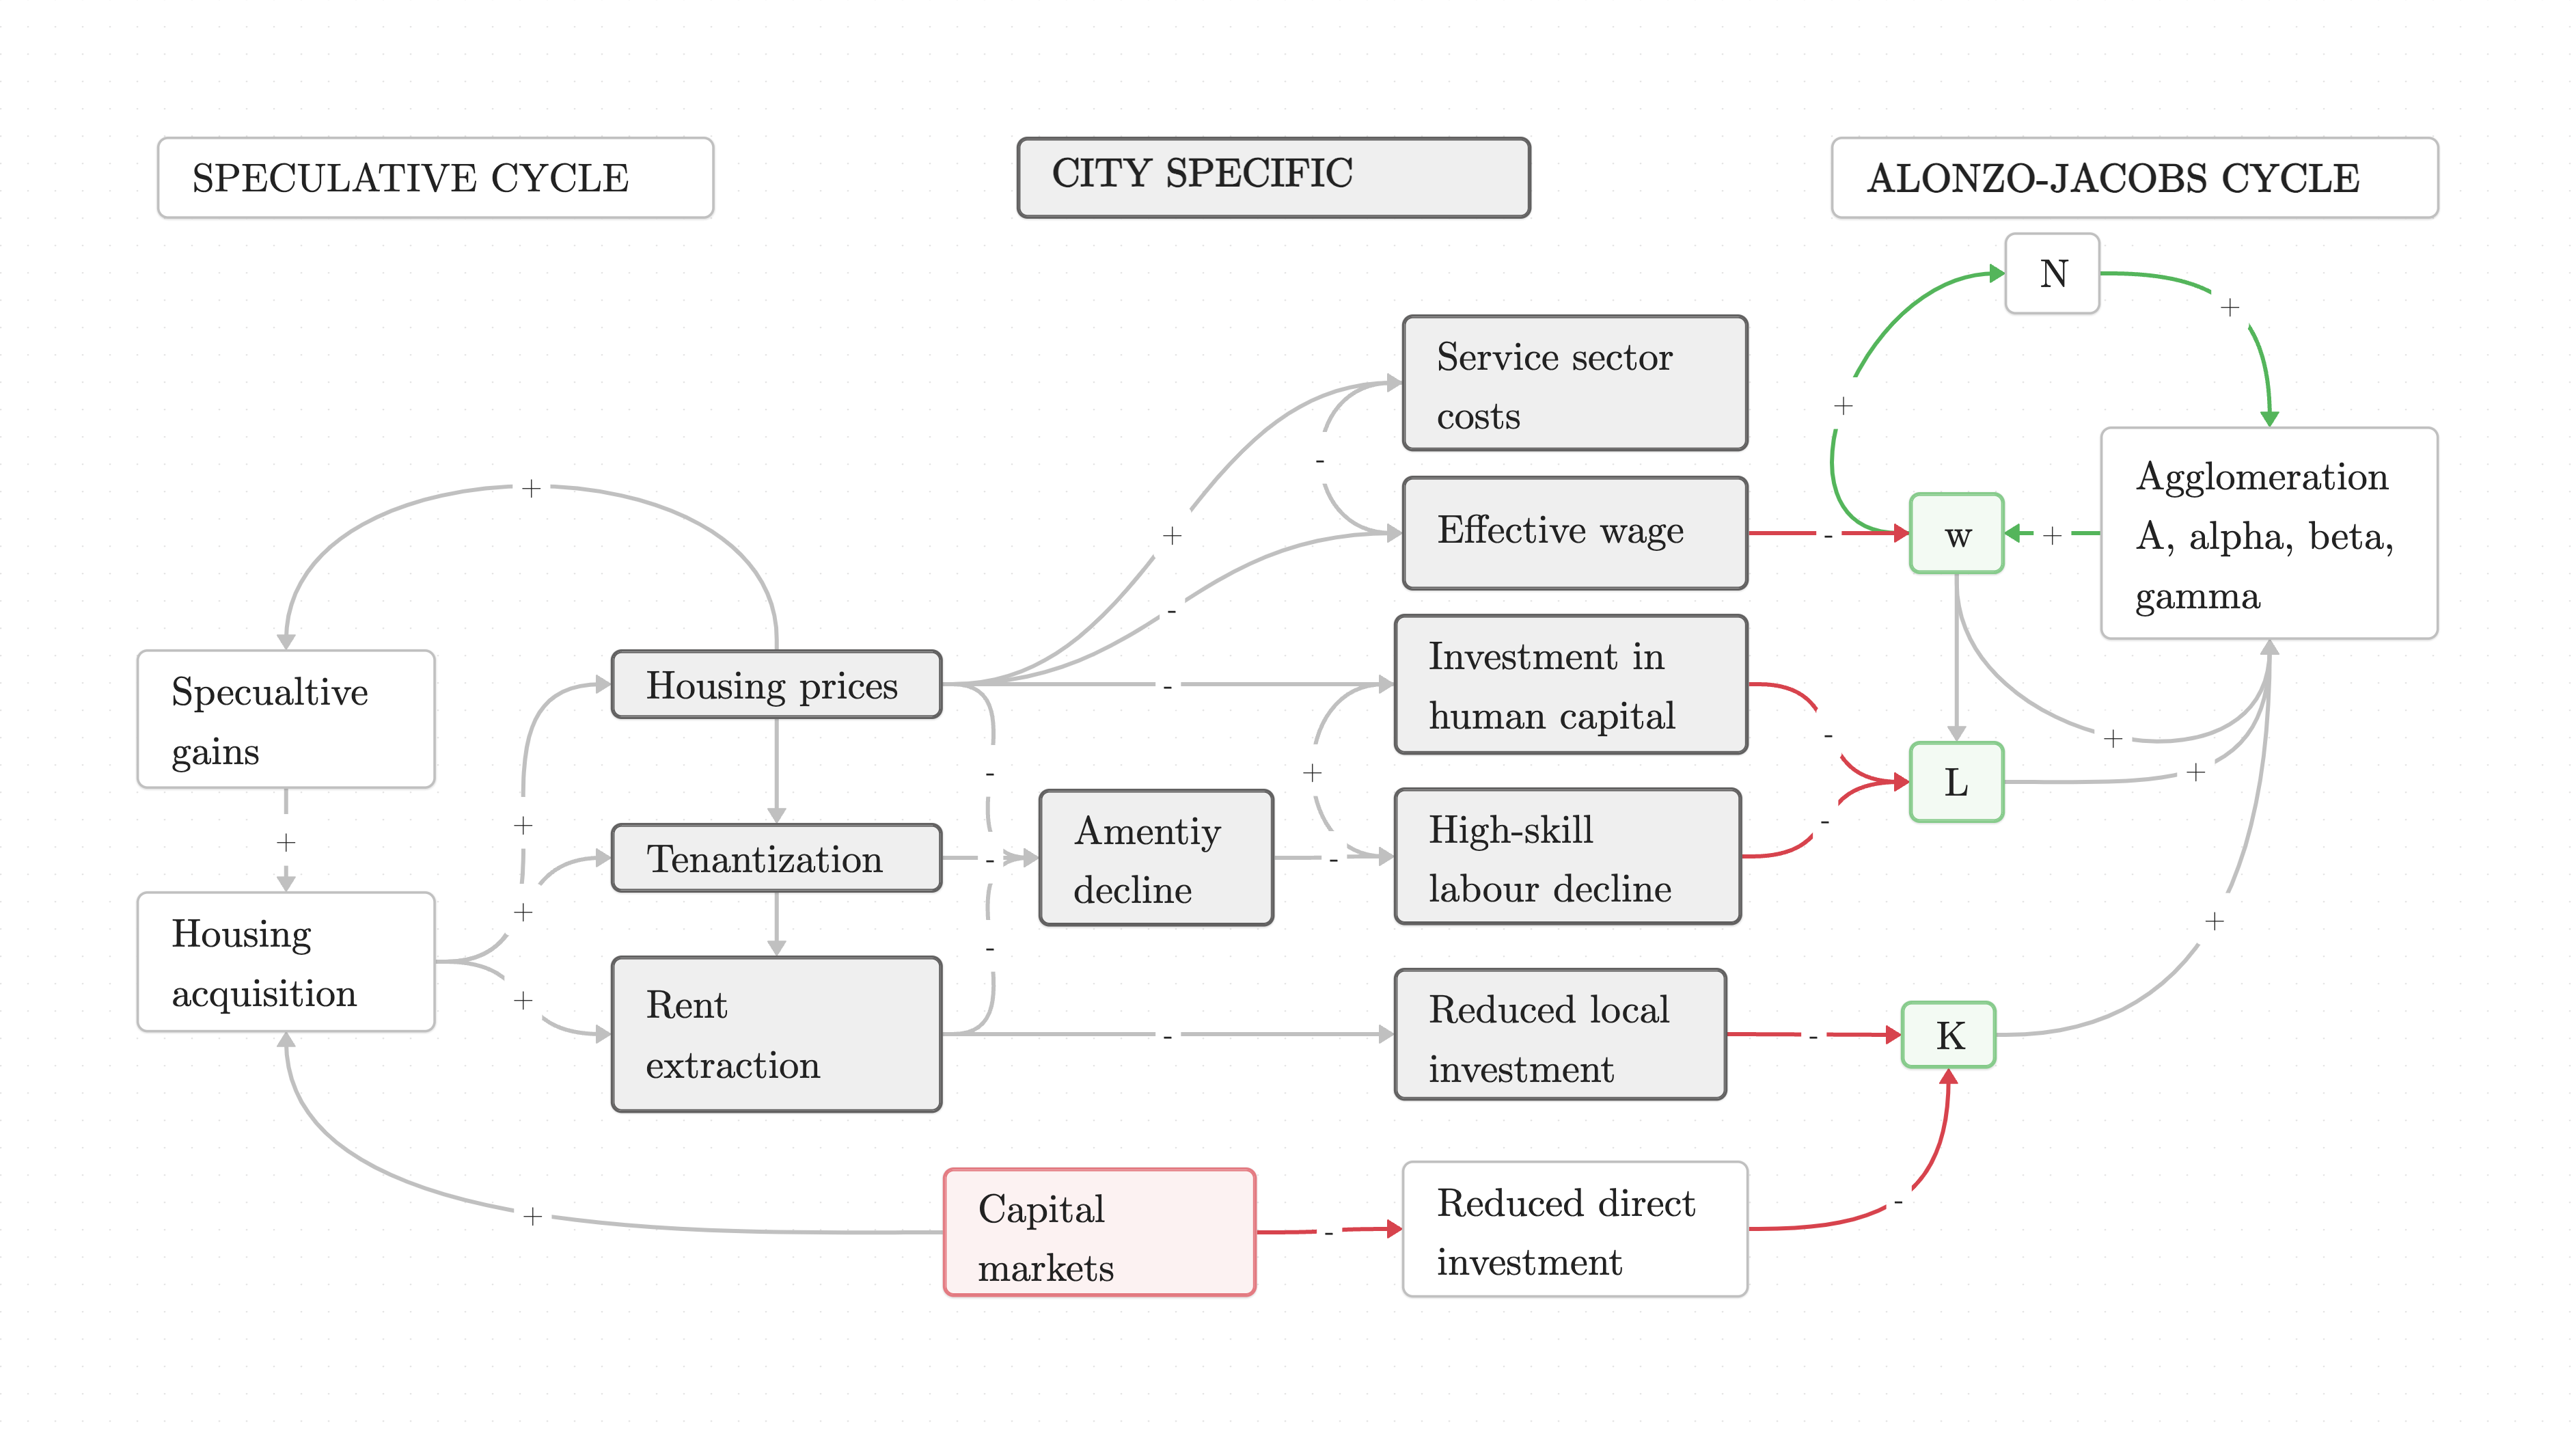
\includegraphics[scale=.15 ]{fig/impact-channels.png}%angle=90
\end{adjustwidth}
\caption{Impact channels relating financialization and urban productivity.}
\end{figure}
%}

There are multiple and variable channels that in theory might link financialization to the magnitude of agglomeration effects in different regions. Figure~\ref{fig-impact-channels} illustrates some of these potential channels.\footnote{The figure shows only some of the links and feedbacks we discuss. Each of the linkages shown or mentioned warrants extensive research, and for most even a brief literature search will reveal many related papers.} 
In the figure, the production sector is on the right, the processes occurring within the city are central, and the speculative intervention in the housing market is to the left. In the upper right, we show the \gls{Alonzo-Jacobs cycle}, described in Chapter~/ref{chapter-model}. In the Alonzo-Jacobs cycle, the strength of the agglomeration effect determines productivity, which in turn drives wages, which determines population which feeds back to agglomeration. In our model, anything that affects productivity must work through the parameters $A$, $\alpha$, $\beta$, or $\gamma$ or through factor supply. 

Any negative effect on urban productivity can have significant consequences at the national level. Over 80 percent of Canadians live in urban centres. Two-thirds of the economic growth in Canada was generated in its six biggest metropolitan areas and about 80\% of the growth comes from the urban areas in total \cite{w.fanImportanceCitiesEmphasis2010}. A reduction of 1.5\% in the productivity growth of these six large metropolitan areas alone would reduce the national growth rate by 1\%. Over 40 years the loss would be equivalent to 33\% of current GDP.

If any of the channels we describe below are significantly affected by financialization, Governments may be able to increase social wealth and well-being through policy instruments at affect the level or impact of financialization. 



%making it indistinguishable from the Jacobs model at the urban level. 
%In addition, the variation suggests that  financialization may have an impact through multiple channels.  


%{\color{red} In the next section we discuss potential linkages  with reference to the two dominant theoretical frameworks for understanding agglomeration effects, %. Second, it introduces the micro-foundations, the mechanisms by which agglomeration happens, drawing on the literature, and discussing how financialization might affect those mechanisms. Finally, in section~\ref{section-impact-channel-summary}, we summarize the primary linkages as they might appear in our model.} 

% {\color{red}WHAT IS AN IMPACT CHANNEL, WHY ARE WE ASKING THIS - BY WHAT MEANS. FINACIALIZATION DOES THIS, PRODUCTIVITY IS THIS. THERE IS NOT NECESSARILY A CONNECTION, BUT THERE ARE CONNECTIONS. 
% Not one is dependant on another necessarily, but they are related in these ways.
% They are two distinct things that are not necesarily conected, but it does seem likely there i s an impact, so what are the channels. 

% Why are they seperate 
% urban productivity involves this feature this featuer this featuer
% financialization of the housing system has this feature this feature and this feature...

% MOST IMPORTANT THINGS

% ADD WHERE WERE GETTING THIS INFORMATION..- SAY WHAT THE SOURCES ARE..
% }

\section{Channels through which financialization may affect productivity}
The literature on financialization generally focuses on the housing market and the social consequences of rising home prices and tenantization.  Relatively few researchers discuss the several possible mechanisms by which financialization might affect the productivity of the city. The fairly preliminary typology we present below is intended to establish that links between financialization and productivity should be explored. We believe that the arguments in this section do establish the plausibility of linkages, but, perhaps because researchers have not looked for links, there is not a body of empirical work to draw on. We will show evidence in our results section that further research on these linkages would be valuable.

%theory suggests a relationship that has not been observed, modelling can help identify the kind of evidend.%ANY THING OVERARCHING WE CAN SAY ABOUT THIS?LATER, IN CONCLUSION YOU SAY : To do this, we identified the housing market channels through which the changes in ownership might be transmitted through the economic and social body of of the city to the Alonso-Jacobs cycle, where agglomeration effects generate wealth.  

\subsection{Reduced capital stock}

Marxist theorists \cite{lefebvreRevolutionUrbaine1970, harveyClassmonopolyRentFinance1974, harveyUrbanProcessCapitalism1978, christophersRevisitingUrbanizationCapital2011} have argued that finacialization diverts capital investment from productive investment to financial enterprises. 

This direct effect is illustrated at the bottom of Figure~\ref{fig-impact-channels}, where capital markets can divert capital from the productive activities on the right to speculative activities on the left.  Switching happens in response to the relative rates of return on the two sides. We have assumed a perfectly elastic supply of capital to firms and speculators, leaving modelling more complex and possibly more realistic capital markets to later work.  We allow the rate of return on housing investment to rise in response to city growth, however, attracting speculative investment. We could also simulate a falling rate of return on non-housing investment by reducing the cost of capital to investors or by inhibiting the rate of growth of capital on the production side in response to rising investment in housing purchases. % adjK


\subsection{Local investment}

Financialization may reduce the amount of local capital available, raising the cost of capital in the city. 
There are at least two mechanisms by which local investment capital may be affected. First, if increased tenantization and rent extraction reduce household wealth, we would expect household investment to decline. The decline would probably be correlated with a decline in direct investment, amplifying its effect. Furthermore, this channel would act very slowly and persist after an initial round of speculative activity. 

Second, because private production is complemented by public infrastructure, it is possible that the tenantization for the city would lead to declining municipal investment in public infrastructure. It is known, however, that municipalities generally spend less on tenants and collect more revenue per capita from rental as opposed to owner-occupied housing, so tenatization might lead to rising pressure for infrastructure expenditure.  We can capture these effects by linking the owner-occupier ratio to capital stock. A more detailed approach would explicitly allocate some of the municipal taxes to increasing the agglomeration parameters.


\subsection{High-skill labour decline}

 Speculation and rising housing prices that result in tenantization will make a city less attractive to highly skilled labour, making it more difficult to attract or hold people with the specific adaptive skills Glaeser and Saiz \cite{glaeserRiseSkilledCity2003} identified. Slowing in-migration or increasing out-migration of the more skilled members of the labour force  will \textit{ceteris paribus} reduce the effective supply of labour. 
Liu et al \cite{liuImpactUrbanHousing2023}, for example, found for China that an increase in urban housing prices has a crowding-out effect on labour mobility.  Duffy et  \cite{duffyRisingHousePrices2005} found that for Ireland that rising house prices, by discouraging potential migrants, could significantly reduce the growth potential of the economy, shifting the balance of labour market growth from employment to wages, with a consequent deterioration in competitiveness. %Anecdotal evidence comes from comes form the frequent news stories about which cities are most livable: low housing prices are almost always an important element in the measures used. (we omit the link form  housing prices to high-skill labour. 

Althobaiti et al \cite{althobaitiHousingPricesSkills2021}  show that with gentrification, high-level cognitive skills are getting closer to the city center in response to the increase of median housing prices while low-level physical skills got further away.  Gentrification can be seen as trend opposing tenantization. The effects of tenantization, neighborhood decline and disinvestment, which Cornelissen and Jang-Trettien \cite{cornelissenHousingContextNeighborhood2023} point are more common than gentrification in low-income neighborhoods, are likely to be opposite of the effects of gentrification.

The reduction might be offset by importing human capital, though immigration or rising wages for talent in the city. Florida\cite{floridaCompetingAgeTalent2005, floridaCreativeClassEconomic2014} has suggested that urban growth is strongly linked to the ability to attract talent. 

We can introduce this channel by making the labour elasticity of output in the Cobb-Douglas function, $\beta$, depend on the home-ownership ratio.  


\subsection{Reduced investment in human capital}

There is a vast literature on investment in human capital. 
Growth theory associates increasing returns to scale in the industrial sector or at the national level with increasing effective human capital, which grows faster than the labour supply as a result of increased education, as we described in Chapter~\ref{chapter-growth} section~\ref{section-growth}. 
Growth theory suggests that the growth of human capital is  a major driver of productivity.  At the national level, Solaki \cite{solakiRelationshipEducationGDP2013} demonstrates a causal relationship between education and growth, and that tertiary Education should be considered as an exogenous variable.  Empirical results for Bangladesh \cite{islam2007relationship}show evidence of bidirectional causality between education and growth.  Among others, B\"uchler et al have recently confirmed the important of human capital growth for urban growth.

There are at least two mechanisms by which investment in human capital may be affected indirectly by financialization. The most direct is by reducing household incomes The effect may be different for different parts of the population. Increasing housing prices increases the wealth of owner-occupiers. this wealth effect may result in increased spending on education for offspring. Increased housing costs for tenants, on the other hand,  may result in reduced human capital investment.\footnote{Glaeser and Saiz found evidence for skill upgrading in declining cities, which suggested to them efficient investment in less skilled workers is a key adaptive/growth mechanism. If powerful enough this effect might offset some of the negative impacts of financialization we has suggested.}  

Less directly, we suspect financialization will increase the cost of living through, for example, increasing labour costs in the service sector. This results in a reduction of the effective wage, also reducing income available for human capital investments. Rent capture leading to reduced local capital of reinvestment in human capital might reduce the adaptive capacity of a city's population.

We can simulate some human capital effects simply by making a link from the home-ownership ratio to the productivity parameters  $\beta$ and $A$. 

\subsection{The effective wage}

Purchasing power depends on the money wage and on the price level. inflation coming from the right side of the figure will reduce the effective urban wage, which Lobo et al. find is one of the determinants of growth. 

 Rising housing prices and rising rental prices reduce the purchasing power of city dwellers in more than one way. In addition to the direct effect, the rising housing costs make other goods and services more expensive. The wage of the Barista must go up, so the cost of a coffee has to rise. Bookstores may close, reducing the neighbourhood amenity level. 
 
 Local amenities may also be affected. Urban amenities  are part of the incentive for choosing city life for many, and any decline in amenity will have the same qualitative effect as a decrease in the wage. The size of the effect will vary because people's tastes differ. 


 General financialization may also reduce the bargaining power of labor, as Tomaskovic-Devey and Lin argue \cite{tomaskovic-deveyFinancializationCausesInequality2013}, reducing wages.\footnote{Tomaskovic-Devey and Lin point to a shift in behaviour of non-finance firms away from production and non-financial services and toward financial investments and services. This shift, they argue,  has led to lower employment, income transfers to executives and capital owners, and increased inequality among workers \cite{tomaskovic-deveyFinancializationCausesInequality2013}}
%In the second part of the chapter we implement several of the mechanisms and share results. 

% VERY INTERESTING \cite{buchlerImpactHumanCapital2024} in areas with elastic housing supply, the positive demand shock leads to the construction of more housing, a larger labour force, and, thus, moderate wage growth. In contrast, in areas of low housing supply, the positive demand shock has a limited impact on new housing construction and the urban population. Human capital gets capitalised into higher home prices, hindering urban growth.

\subsection{The amenity channel}
Rent capture might influence the concentration of educated personnel by reducing the diversity and amenity of cities, making urban living less attractive, reducing labour supply, or raising its cost.



\subsection{Impact on the service sector}
Rising housing costs at the centre of a city would tend to push low-wage workers to the edges, increasing their transportation costs, putting further upward pressure on wages, and increasing the costs of all amenity services that rely on lower-cost workers.


\section{Conclusion}
 The dominant effect of financialization is to shift ownership of housing from occupiers to owners of financial capital. In this chapter, we have described a number of the most likely channels through which the effect of financialization might be transmitted to the Alonso-Jacobs cycle, where agglomeration effects generate wealth. Our list is not complete but it provides theoretical grounds for testing the model's sensitivity to a range of policy interventions and lays the foundation for empirical work.  

 Understanding the mechanisms has considerable policy importance because it raises the possibility that there are several channels for public policy to enhance the positive effects of agglomeration. Determining the importance of the various impact channels in general or for a specific city is an empirical problem well outside the brief of this thesis but tests in the universe of the model can lay the foundation for later empirical work.  In the Chapter~/ref{chapter-model} we therefore present a model in which we can systematically test the model's sensitivity to a range of policy interventions if any spillovers to productivity of the type we discuss here exist. In the results section we will further explore, based on our analysis and simulations, how the unrecognized impacts of financialization of the urban housing market may have extremely serious effects on the economy as a whole. 

%Financialization may indirectly affect urban productivity at many points in the system. We defer extending the model to include these effects. Our focus in this chapter has been limited to examining possible channels through which the housing market financialization is likely to affect the productivity of a city. 

% We have modeled the relationship between ownership and the inputs to the aggregate production function described in Chapters~\ref{chapter-growth} and \ref{chapter-model}. 

% {\color{red}
% Essentially, the discussion in this chapter has guided and helps explain the policy experiments we have conducted. MAYBE ADD A FINAL SENTENCE PULLING IT ALL TOGETHER?}




% \subsection{TODO ADD BACK MOVE TO TRANSMISSION CHAPTER? The transmission puzzle}

% %The transmission of productivity increases arising from agglomeration effects  to the urban wage through firms, can be modelled in many ways. The agglomeration effects are external to the firm and therefore likely to be unexpected. If  firms underestimate the marginal product of labour, labour productivity will be greater than expected, output will be higher than planned output, and revenue and profits will therefore be higher than expected. Excess demand will attract more productive capital which in turn will demand more labour,  Rising labour demand drives up the wage. The agglomeration effect driving growth is essentially a public good in which individual firms will under-invest. This raises a policy challenge that we leave for others. CLARIFY - ALSO STILL A FOOTNOTE IN MODEL SECTION. CUT OR REF THEiR IF MOVING HERE.

% % It is straightforward to compute the rate of excess return for  this model. 

% %
% \begin{figure}
% \centering
% 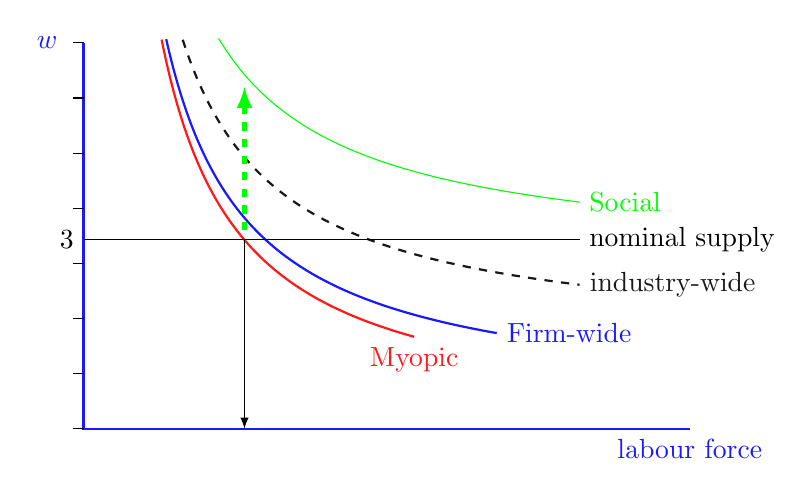
\begin{tikzpicture}[scale=.7]
%\def\bndmax{5}        %https://tex.stackexchange.com/questions/68462/filling-a-complex-region-with-tikz
%\def\bndmin{0.2}
\def \Y {7}  % height of y axis pecent
\def \W {15}  % length  of x axis
\def \Wbar {3} % jmeam wealth
\def \omega {3}
\def \A {1}  %was .5
\def \B {.5}

\draw [thick, color=blue!90] (0,\Y)node[left=.2cm]{$w$} -- (0,0)--(\W-4,0)node[below]{labour force};  
 \foreach \yi in {0,...,\Y} \draw (0,\yi)--(-.2,\yi)node[left]{};
 
\tikzset{func/.style={thick,  color=blue!90}}
% \draw[ func, domain=.2:\W-6] plot [samples=200] (\x, 2*\x^.5)node[below=.1, right]{SUPPLY};

\tikzset{func/.style={  color=green}}	
\draw[func, domain=2.45:\W-6] plot [samples=200] (\x, 10/\x+3)node[above=.1, right]{Social};

\tikzset{func/.style={thick, dashed, color=black!90}}	
\draw[func,domain=1.8:\W-6] plot [samples=200] (\x, 10/\x+1.5)node[ right]{industry-wide };

\tikzset{func/.style={thick, color=blue!90}}	
\draw[func,domain=1.5:\W-7.5] plot [samples=200] (\x, 10/\x+.4)node[below=.05, right]{Firm-wide};

\tikzset{func/.style={thick,color=red!90}}	
\draw[func,domain=8.5/6:\W-9] plot [samples=200] (\x, 10/\x)node[below]{Myopic};

\draw[](0,3.425)node[left]{$\omega$}--(9,3.425)node[right]{nominal supply };
\draw[thin,latex-](2.92,0)--(2.92,3.425); %a vertical labour supply
\draw[ultra thick,dashed, green,-latex](2.92,3.6)--(2.92,6.2);
%\draw [blue,  thick](13, 8.3)--(15,8.3)node [right, black] {\small A=\ 1,\ B=0.5};
%\draw [green, thick](13, 7.6)--(15,7.6)node [right, black] {\small A=.8, B=0.8};

%\node at (5,-1.5){Resulting in  profits, expansion, and/or entry: the city grows};
 \end{tikzpicture}
% \caption{Multiple marginal products.}
% \label{fig-multiple-marginal-products}
% \end{figure}



% %5Figure~\ref{fig-marginal-products} illustrates the problem. We can  make a distinction between the myopic marginal productivity curve observed  at the shop floor level and  the firm-wide effect of adding a worker. The red curve labeled ``Myopic'' represents the declining direct marginal productivity of labour as  might be observed by a shop manager, who could report how much more output one with one worker one lathe would produce. The blue line above it labeled ``Firm-wide'' represents the actual effect on firm productivity that arises because the new worker makes other workers in the firm more productive. This addition to output would be observable for managers reviewing the firm's performance over time. It might be most easily observed in small firms. 

% %We can go on to consider the slower and distributed effect on closely related firms, which would raise any estimate of marginal product.  If there are 10 other firms and a new worker  has a small spillover effect  $\epsilon$ on each,  the spillovers raise the industry  marginal product  by $10\epsilon$. Each of the  10 other firms  enjoys  an additional $10\epsilon$ gain in the marginal product of their workers. This should lead to additional hiring by other firms.

% %Finally, expanding our view another step, we notice that if each of the  10 other firms hires one worker who produces an additional  $10\epsilon$ gain in output for all firms, the total spillover effect would rise by $100\epsilon$. The social marginal product of a single hire is indicated by the green line. 


 
\section{Our linkage model}

THIS WILL BE MOVED TO THE BOTTOM OF MODEL

As we point out in Chapter~\ref{chapter-transmission} there are two types of effect - a reduction in the inputs to production, labour and capital, and a change in the parameters of the production function, $A$, $\alpha$, $\beta$,or $\gamma$.  These are not perfectly distinct. Technology is not an explicit input in our model as it is in the growth literature described in Chapter~\ref{chapter-growth}. It has been subsumed into the parameter $A$. Public inputs, like the transportation system do not appear directly any of the models, so that their effect is likely to affect estimates of $A$ and also to  inflate the residuals. We  use these observation to justify our specific implementation. 

The scale parameter $A$ controls the overall productivity of the urban system. It captures several productivity-enhancing effects: the contribution of urban infrastructure, ownership participation by residents, local investment in productive capital, regulatory structure, the presence of local universities, the skill level of the workforce, as well as other factors. 

Since we are interested in the effect of financialization and ownership, we rewrite $A$ as:
\[ A= A_0 + share * rent\]
$A_0$ represents outside or general factors contributing to productivity, while $share*rent$ stands for the share of the urban locational rents captured by residents and contributing to local productivity\footnote{that there are local factors is indicated by the variability of estimates of $A$ in empirical studies. See Subsection~\ref{fig/sec-fig-resiudals}.}. The share term is itself a composite of the actual land-ownership share of residents determined by the housing market and the propensity to invest locally.  It might contribute to overall productivity through several channels we discuss below:  directly through investments that raise productivity in firms, indirectly through investments in urban infrastructure such as transportation that cuts production, or through other channels such as workforce improvements. 

The effect of varying $A$ can be seen in Figure~\ref{fig:generic-productivity-impact}  

